\documentclass[11pt]{article}
\usepackage[a4paper, hmargin={2.8cm, 2.8cm}, vmargin={2.5cm, 2.5cm}]{geometry}
\usepackage{graphicx}
\usepackage[utf8]{inputenc}
\usepackage[square]{natbib}

\author{
    \begin{tabular}{ccc}
    \Large{August V. S\o rensen} & \& & \Large{Magnus N. Stavngaard} \\
    august.vinkel@gmail.com      &    & magnus@stavngaard.dk
    \end{tabular}
}

\title{
    \Huge{Authorship Verification} \\
    \Large{Deep Learning Based Methods for Authorship Verification}
}

\usepackage{fancyhdr}
\pagestyle{fancy}

\lhead{University of Copenhagen}
\rhead{August V. S\o rensen \& Magnus N. Stavngaard}

\begin{document}

    \maketitle

    During the last 6 months, we have created a system designed to determine if
    a secondary school student has used a ghostwriter on a text he/she turned in
    via Lectio. The system we developed is intended to be a tool that assists
    teachers in more accurately determining the authenticity of an assignment,
    while also providing a description of what factors contributed to the
    decision the system made.

    We were given two goals: To keep the number of false accusations the system
    made below 10\% and to catch 95\% of the ghostwriters. Keeping a low amount
    of false accusations was the primary goal of the two, meaning that the focus
    of the experiments were on keeping false accusations below 10\% while
    catching as many ghost writers as possible.

    This summary will go through the major points of our thesis. If any more
    information is desired, please refer to the full thesis. Of special
    interest to you is probably Section 1 (Introduction), Section 5.2 (Deep
    Learning), Section 7.1 (Results), Section 7.2 (Teacher Feedback), Section
    7.3 (Applicability of Method) and Section 8 (Conclusion).


    \section{The System}

    The networks we developed is trained to compare two texts. The network will
    report the probability that the two texts are written by the same author.
    Since students have normally written more than one text, we also developed a
    method for combining the output of the networks on multiple texts.

    When we are testing whether a text is ghost written or not, we compare it to
    all texts we know to be written by the student (his/her previous turned in
    texts). We then combine the probabilities the network gives for each text.
    We found by experimentation that the best way of scoring the probabilities
    is to consider the length of the texts and when the texts were turned in.
    Newer texts gives a better estimate of an authors writing style than older
    texts. Similarly longer texts gives a better estimate of an authors writing
    style than shorter texts. We have illustrated how our implemented methods
    works in Figure \ref{fig:model}.

    \begin{figure}
        \centering
        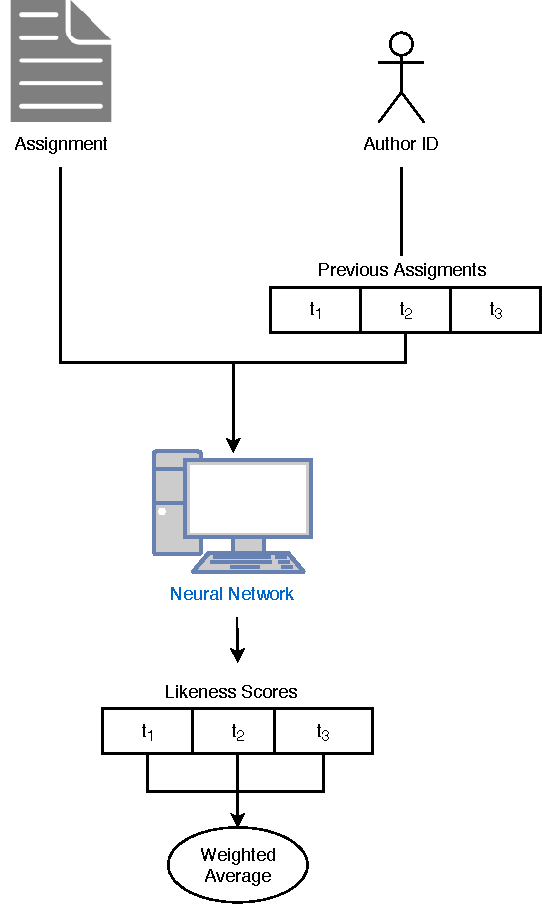
\includegraphics[width=0.5\textwidth]{./pictures/Model}
        \caption{Illustration of how a new text is verified to be written by an
            author or a ghostwriter. The input is a new text and a
            \textit{candidate} author of the text. The candidate is represented
            by a set of texts he/she has written before. We compute the
            similarity between the new text and all older texts. The
            similarities are combined to give a final prediction on whether or
            not the assignment is ghostwritten.}
        \label{fig:model}
    \end{figure}

    We control the number of false accusations the system makes by changing the
    threshold for when we say an assignment is ghostwritten. The output of the
    weighing scheme described above is a single number between 0 and 1. When it
    is close to 1 the authors writing style is very close to the new text and
    when it is close to 0 it is very dissimilar. By choosing a low threshold
    such as 0.1 we make sure that writing style has to be very dissimilar before
    we accuse anyone of using a ghostwriter.


    \section{Results}

    We evaluated our networks on two datasets. A dataset containing 50\%
    ghostwritten texts and a dataset containing 4\% ghostwritten texts. We used
    the 50\% dataset since previous work on your dataset used that and we wanted
    to directly compare our results to previous work. We used the 4\% dataset
    since that reflects the believed number of ghostwritten SRP assignments in
    the real world.

    It is much harder to obtain a low accusation error on a dataset with
    only 4\% ghostwritten texts. For each assignment there is a chance we
    make a mistake so if there are 19 non ghostwritten texts for each single
    ghostwritten texts there is a larger possibility of making mistakes on non
    ghostwritten assignments than if the ratio was 1 to 1. That means that we
    are forced to lower the threshold we use to a level where we almost don't
    catch any ghostwriters.

    On the 50\% dataset we obtained an accusation error of 6.3\% while catching
    66.0\% of the ghostwriters. On the 4\% dataset we obtained an accusation
    error of 23.5\% while catching 8.5\% of the ghostwriters.


    \section{Teacher Feedback}

    We looked at what kind of feedback we can give to teachers on why we
    consider a text ghostwritten. We only performed these experiments on the
    network that performed best. It was through these experiments we found
    that we were able determine which paragraphs of a text is most likely
    ghostwritten. This would allow a teacher suspicious of a student to identify
    paragraphs of assignment to focus on.

    What the network looks at when making a decision is the presence or absence
    of certain phrases in the texts it is comparing. An example of such a phrase
    is "F. eks.". Some students often use that abbreviation while others do not.
    Therefore it is a sign that a different author wrote the assignment if that
    suddenly changes. We are able to report the largest differences between two
    assignments by the presence and absence of hundreds of such strings.

    Individually they are useless in explaining why an assignment is
    ghostwritten but if hundreds of them suddenly changes that is a clear
    sign that a ghostwriter might have been used. A teacher can get access to
    the phrases that changed between two assignments and possibly use that
    information for explaining why an assignment is ghost written.


    \section{Conclusion}

    We believe that our results are promising. We have obtained slightly better
    results than previous work on your dataset that we have found (comparing
    results on a 50\% ghostwritten dataset) \citep{hansen2014,aalykke2016}. But
    we also believe that our methods require more work before they are ready for
    implementation (based on the results on the dataset with 4\% ghostwritten
    texts). We don't believe that it is possible to both achieve an accusation
    error of less than 10\% while also catching 95\% of cheaters. However, we
    do believe that with further work it would probably be possible to catch
    10 to 20\% of the cheaters while keeping the accusation error below the
    threshold.

    \newpage
    \bibliographystyle{apalike}
    \bibliography{literature}

\end{document}
